\documentclass{amsart}
\usepackage[foot]{amsaddr} % put addresses on first page

\usepackage{geometry}
\usepackage{graphicx,psfrag,epsf}
\usepackage{enumerate}
\usepackage{enumitem}
\usepackage{amsfonts}
\usepackage{mathtools}
\usepackage{amssymb}
\usepackage{amsmath}
\allowdisplaybreaks
\usepackage{longtable}
\usepackage{bigints}
\usepackage{siunitx}
\usepackage{amsthm}
\usepackage{soul}
\usepackage{color}

\usepackage{hyperref}
\usepackage[capitalise]{cleveref}
\newtheorem{theorem}{Theorem}[section]
\newtheorem{corollary}{Corollary}[theorem]
\newtheorem{lemma}[theorem]{Lemma}
%

\usepackage[numbers]{natbib}
\usepackage{url} % not crucial - just used below for the URL 
\usepackage{doi}

\title{Copula estimation using loss-based Bayesian Additive Regression Trees}
\author{**}
\date{\today}

\begin{document}

\maketitle

\section{Introduction}

\section{Model}
Let $Y_1$ and $Y_2$ be two continuous random variables and $X$ be a continuous random variable 
that might affect the relationship between $Y_1$ and $Y_2$. 
Then according to Sklar’s theorem there exists a unique copula such that:
\begin{equation}
    H_{X}(y_1,y_2\mid x; \theta, \alpha_1, \alpha_2) = C\{F_{Y_1\mid X}(y_1\mid x;\alpha_1),F_{Y_2\mid X}(y_2\mid x; \alpha_2)\mid x;\theta\}; \quad \forall (y_1,y_2) \in \mathbb{R}^2.
\end{equation}
This gives us the following
\begin{equation}
    h_{X}(y_1,y_2\mid x; \theta, \alpha_1, \alpha_2) = f_{Y_1\mid X}(y_1\mid x;\alpha_1)f_{Y_2\mid X}(y_2\mid x; \alpha_2)c(u_1,u_2\mid x;\theta),
\end{equation}
where
\begin{equation}\label{eq:emp_dist:Y}
    u_k = F_{Y_k\mid X}(y_k\mid x; \alpha_k)
\end{equation}
and $c(u_1,u_2\mid x;\theta)$ is conditional copula density function.

\subsection{Copula parameter estimation}

Let $\Phi_{\theta\mid x}(y_1, y_2)$ denote the standard bivariate normal distribution with correlation coefficient $\theta$ conditional on $X$. Then
the corresponding copula density function is given by:

\begin{equation}
    c(u_1,u_2\mid x;\theta) \coloneqq c_{\theta_x}(u_1, u_2) 
    = \frac{1}{\sqrt{|\Sigma|}} \exp\left( -\frac{1}{2}
    \begin{bmatrix}
    \Phi^{-1}(u_1) \\
    \Phi^{-1}(u_2)
    \end{bmatrix}^\top
    (\Sigma^{-1} - I)
    \begin{bmatrix}
    \Phi^{-1}(u_1) \\
    \Phi^{-1}(u_2)
    \end{bmatrix}
    \right)
\end{equation}

where

\[
\Sigma = \begin{bmatrix}
1 & \theta_x \\
\theta_x & 1
\end{bmatrix}
\]

and \( \Phi^{-1} \) is the inverse of the standard normal cumulative distribution function. Simplifying we get:

\begin{equation}
    c_{\theta_X}(u_1, u_2) = \frac{1}{\sqrt{1 - \theta_x^2}} \exp \left( -\frac{2\theta_x \Phi^{-1}(u_1) \Phi^{-1}(u_2) - \theta_x^2\left[\Phi^{-1}(u_1)^2 + \Phi^{-1}(u_2)^2\right]}{2(1 - \theta_x^2)} \right)
\end{equation}

Now, let $u_1 \coloneqq (u_{11}, u_{12}, \cdots, u_{1n})$ and $u_2 \coloneqq (u_{21}, u_{22}, \cdots, u_{2n})$ be a set of $n$ observations from a bivariate
Gaussian copula.


Then, the likelihood is given by:

\begin{align}
    \pi(U_1, U_2\mid X;\theta_x) &=\prod_{i=1}^n  
    \frac{1}{\sqrt{1 - \theta_{x_i}^2}} \exp \left( -\frac{2\theta_{x_i} \Phi^{-1}(u_{1i}) \Phi^{-1}(u_{2i}) - \theta_{x_i}^2\left[\Phi^{-1}(u_{1i})^2 + \Phi^{-1}(u_{2i})^2\right]}{2(1 - \theta_{x_i}^2)} \right)
\end{align}
where for a tree $T$ with terminal node values $M$
\begin{equation}
    \theta_{x_i} = g(x_i, T, M)
\end{equation}
Now, terminal node values $M \coloneqq (\mu_1, \mu_2, \cdots \mu_{n_L})$ has to
satisfy $\mu_j \in (-1,1)$. This leads to the issue of finding a suitable prior 
for $\mu_j$.

Note that the likelihood structure for a partition $\Omega_j$ of $x\coloneqq (x_1, x_2, \cdots, x_n)$

\begin{align}
    \pi(U_1, U_2\mid X;\theta_x) 
    &=(1 - \theta_{x}^2)^{-\frac{\#\Omega_j}{2}} \exp \left( -\frac{2A \theta_{x} - B\theta_{x}^2}{2(1 - \theta_{x}^2)} \right)
\end{align}
where $A \coloneqq \sum_{i\in \Omega_j}\Phi^{-1}(u_{1i}) \Phi^{-1}(u_{2i})$
and $B \coloneqq \left[\Phi^{-1}(u_{1i})^2 + \Phi^{-1}(u_{2i})^2\right]$. 

\subsubsection{Choice for $\mu_j$}
\begin{itemize}
    \item Jeffrey's prior \url{https://www2.stat.duke.edu/~berger/papers/bivariate.pdf}
    \item Simple uniform distribution in $(-1,1)$ 
    \item Transformed beta \url{https://academic.oup.com/jrsssa/article/145/2/237/7105492}
    \item Log-normal on $-\log(1-p^2)$
    \item Inverse-Gamma on $-\log(1-p^2)$
\end{itemize}
Note that for the first three choices, we only work with transformed beta distribution by 
selecting suitable hyper-parameters.

\section{Simulation Studies}

We consider 5 different test cases so that
\begin{itemize}
    \item True $\theta_x$ has a tree structure with respect to $x$
    \item True $\theta_x$ is monotone with respect to $x$ such that 
    \begin{equation}
        \theta_x = 0.5 + 0.2 \sin(3x) + 0.3x^2
    \end{equation}
    \item True $\theta_x$ is convex with respect to $x$ such that 
    \begin{equation}
        \theta_x = 0.6 + 0.3 \sin(3x)
    \end{equation}
    \item True $\theta_x$ is concave with respect to $x$ such that 
    \begin{equation}
        \theta_x = 0.9 - 0.3 \sin(3x)
    \end{equation}
    \item True $\theta_x$ non-convex and non-monotone with respect to $x$ such that 
    \begin{equation}
        \theta_x = 0.7 - 0.3 \sin(2x) + 0.2 \sin(4x) + 0.3 x^2
    \end{equation}
\end{itemize}

\begin{figure}
    \centering
    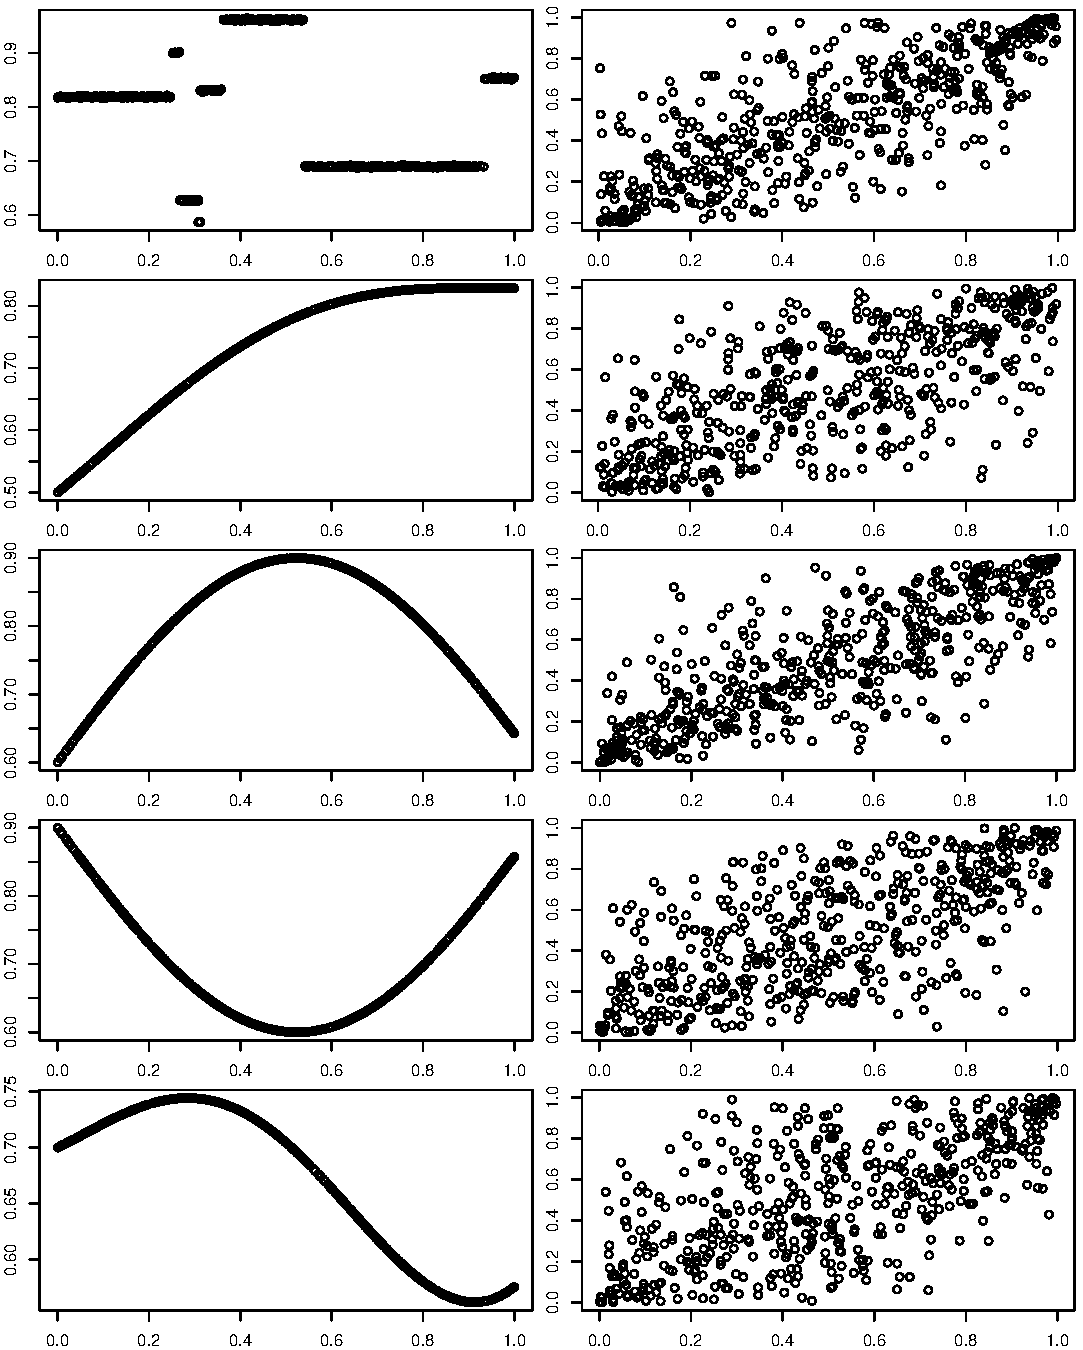
\includegraphics[width=0.95\linewidth]{true_rho_copula.pdf}
    \caption{Simulated $\rho$ and corresponding copula}
    \label{fig:sim-dat}
\end{figure}

\end{document}
